\section{Requirements} \label{sec:requirements}
This section will describe shortly \emph{where} and \emph{how} we implemented the requirements given by the assignment.

\subsection{Scene Graph elements} \label{subsec:sceneGraph}
\subsubsection*{Custom Model}
For manually composed models we have
\begin{itemize}
	\item Chest (which consists of multiple complex parts)
	\item Trolls
	\item Wizard
	\item Treasure Hunter
\end{itemize}

\subsubsection*{Separate Animations}
\begin{itemize}
	\item Running Troll with moving legs
	\item Wizard swinging his staff
	\item Treasure Hunter moving his hands separately
\end{itemize}
\subsubsection*{Render complex model}
See section~\ref{subsec:customModel}.

\subsection{Materials} \label{sec:Materials}
The wizard, moving lightball, gold (in the chest), trees and the whole fireplace (excluding the particle system) are materials.

\subsection{Texturing} \label{Texturing}
See section~\ref{subsec:customModel}.

\subsection{Illumination} \label{subsec:Illumination}

\subsubsection*{Multiple light sources}
Fire (static), wizard light (static), projectile from wizard (moving and spotlight). \label{spotlight}

\subsubsection*{Spotlight}
See section~\ref{spotlight}.

\subsubsection*{Phong-lighting}
Phong shading is applied to all objects in the scene with the exception of the particle system since it is transparent.

\subsection{Transparency} \label{subsec:transparency}
The particle system uses semi-transparent textures.

\subsection{Camera} \label{subsec:camera}
\begin{description}
	\item[E] for upwards movement
	\item[Q] for downwards movement
	\item[W] forward
	\item[A] left
	\item[S] backward
	\item[D] right
	\item[X] to place an additional tree under the camera
\end{description}

\subsection{Custom model} \label{subsec:customModel}
We had to define one model all by our self, and we chose to do this on the chest in the forest.
Our goal was to provide a model which is separated into tow parts: the lower half of the chest and the upper part.
This allows us to animate the hinge of the chest and let it be opened by a guy finding the treasure.


Figure~\ref{fig:chest} shows the chest as a whole model.
The bottom part was mostly just a cube, but the upper half (the rounding) was rather complex.
It is defined by around 40 vertices.

\begin{figure}[h]
	\centering
	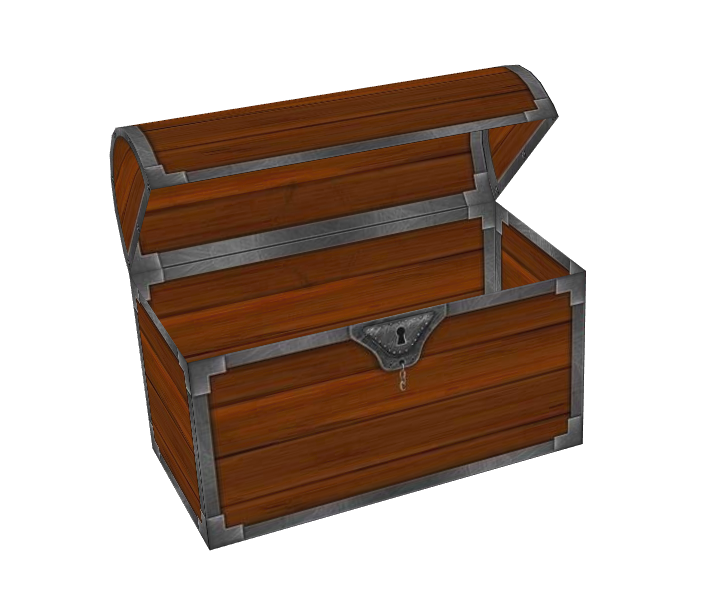
\includegraphics[width=0.5\columnwidth]{figures/chest.png}
	\caption{The chest}
	\label{fig:chest}
\end{figure}

Figure~\ref{fig:chest_side} shows the complex part from the side.
You can clearly see the rounded object.

\begin{figure}[h]
	\centering
	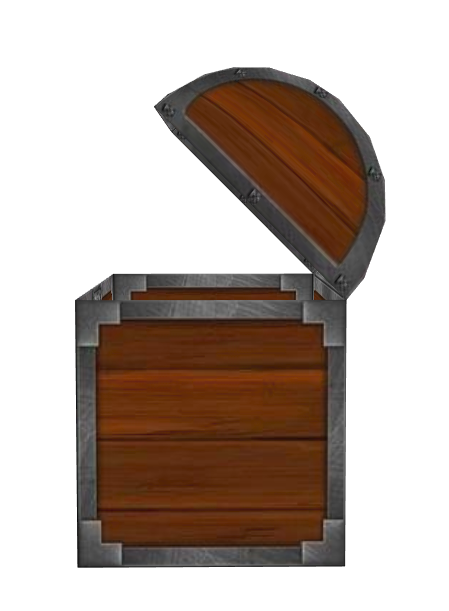
\includegraphics[width=0.5\columnwidth]{figures/chest_side.png}
	\caption{The side view of the chest}
	\label{fig:chest_side}
\end{figure}

\subsection{Alpha texturing} \label{subsec:alphaTexturing}
We added the alpha texture as well alspha belding to our particle system.
More details on the particle system and \emph{alpha blending} are described in chapter~\ref{sec:particleSystem}.
